% Preamble
\documentclass[a4paper, twoside, 11pt]{article}

% Packages
\usepackage[utf8]{inputenc}
\usepackage[english,french]{babel}
\usepackage[a4paper]{geometry}
\usepackage[affil-it]{authblk}
\usepackage{etoolbox}
\usepackage{lmodern}
\usepackage{hyperref}
\usepackage{graphicx}

%%% Biblio %%%

\AtBeginDocument{\setlength\bibitemsep{0.5\baselineskip}}

\usepackage[
    backend=biber,        % compilateur par défaut pour biblatex
%sorting=nyt,          % trier par nom, année, titre
    style=ieee,
    natbib=true
%bibstyle=alphabetic,  % style de bibliographie alphabétique
]{biblatex}
\addbibresource{biblio.bib}

%%% Options taille police titre/auteurs  %%%
\makeatletter
\patchcmd{\@maketitle}{\LARGE \@title}{\fontsize{16}{19.2}\selectfont\@title}{}{}
\makeatother

\renewcommand\Authfont{\fontsize{12}{14.4}\selectfont}
%\renewcommand\Affilfont{\fontsize{9}{10.8}\itshape}

\title{Structured Prediction for Natural Language Processing}
\author{Fronteau T., Jonas W., Lepetit M., Martzloff A., Mousseaux V.}
%\affil{Aix-Marseille Université}

% Document
\begin{document}

 \maketitle
 \section{Similarité sémantique entre phrases}
    L'objectif de ce projet est d'implémenter et d'évaluer un modèle à l’état de l’art pour résoudre une tâche de similarité textuelle sémantique (STS).

    \subsection{Tâche}

        \subsubsection{Campagne d’évaluation SEMEVAL}

    Les campagnes SEMEVAL sont organisées tous les ans et regroupent plusieurs défis en lien avec la représentation du sens du texte. La tâche Interpretable Semantic Textual Similarity a été proposée lors des campagnes d’évaluation SEMEVAL de 2016. Elle consiste à comparer deux phrases en anglais selon leur similarité. Cependant, au lieu de comparer les phrases entières, ici il faut d’abord découper la phrase en segments. En effet, la STS mesure le degré d'équivalence sémantique entre des segments de texte appariés. La STS interprétable (iSTS), quant à elle, ajoute une couche explicative. Étant donné des paires de phrases données en entrée, les participants doivent d'abord identifier les segments dans chaque phrase, puis aligner les segments des deux phrases en indiquant la relation et le score de similarité de chaque alignement, de la manière suivante : \hfill \linebreak
 \paragraph{Étape 1 :}\mbox{}\\
 \begin{eqnarray*}
\textbf{12 killed in bus accident in Pakistan}\\
\textrm{[ 12 ] [ killed ] [ in bus accident ] [ in Pakistan ]}\\
\textbf{10 killed in road accident in NW Pakistan}\\
\textrm{[ 10 ] [ killed ] [ in road accident ] [ in NW Pakistan ]}\\
\end{eqnarray*}
  \paragraph{Étape 2 :}\mbox{}\\
 \begin{eqnarray*}
\textrm{[ 12 ] < = > [ 10 ] : ( SIMILAR 4 )}\\
\textrm{[ killed ] < = > [ killed ] : ( EQUIVALENT 5 )}\\
\textrm{[ in bus accident ] < = > [ in road accident ] : ( MORE-SPECIFIC 4 )}\\
\textrm{[ in Pakistan ] < = > [ in NW Pakistan ] : ( MORE-GENERAL 4 )}
\end{eqnarray*}

 Nous nous contenterons d'établir le score de similarité et n'indiquerons donc pas quelle est la relation (équivalence, implication, ...) entre les segments comparables dans les paires de phrases.

        \subsubsection{Shared Task}
 Dans cette section, nous décrivons les méthodes d'approche et techniques d'apprentissage proposées par la communauté scientifique en réponse à la \og shared task \fg{}.

            \paragraph{DTSim}
        \hfill \break
        Après une phase de preprocessing, Banjade et al. \cite{banjade} utilisent un modèle statistique Conditional Random Fields (CRF) pour la création des segments qui permet de prendre en compte les dépendances entre les différentes prédictions. Pour cela, le modèle utilise notamment comme entrées les mots suivant et précédant le mot courant ainsi que la partie de discours de chacun des trois mots.
Les résultats du modèle CRF sont ensuite enrichis par l'ajout de règles qui permettent d'obtenir des segments plus intéressants d'un point de vue lexical. Le test du modèle présenté comparé à deux autres (\textit{OpenNLP Chunk} et O-NLP enrichi avec les règles ci-dessus) montre que le modèle développé a de bien meilleures performances et que l'ajout de règles permet effectivement la création de meilleurs segments.

 Pour l'alignement des segments, Banjade et al. se base sur un autre modèle développé par Banjade et al \cite{banjadeautre} qui utilise un score de similarité entre les mots pour trouver les segments les plus ressemblants. Un alignement est d'abord effectué entre les mots des deux segments pour déterminer leur score de similarité en utilisant la méthode de Kuhn-Munkres puis un second alignement est effectué afin de maximiser le score. Excepté les outils de preprocessing, l'équipe du projet n'utilise pas de modèle de machine learning se privant ainsi d'outils à fortes capacités et prometteurs en traitement du langage.

        \paragraph{Inspire}
        \hfill \break
Le système Inspire de Kazmi et Schüller \cite{kazmi} repose sur l'utilisation d'un solveur Answer Set, qui utilise une syntaxe et des règles de programmation logique connues sous le nom de Answer Set Programming (ASP). Dans un premier temps, le découpage en segments est effectué en utilisant l'ASP, à partir d'un POS-tagging et d'une analyse syntaxique par transition. Ensuite, l'utilisation d'outils déjà entrainés permet d'associer à chaque segment des caractéristiques en effectuant un POS-tagging, un NER-tagging, un calcul de similarité entre segments à l'aide de Word2Vec, et une recherche de synonymes dans WordNet. Enfin, un ensemble de règles inspirées de NeRoSim terminent de définir le problème ASP, qui est donc résolu sans nécessiter d'apprentissage.

Le système Inspire est dans le top 3 des systèmes présentés lors du concours, pour l'évaluation des bases de données Headlines et Images, mais il est le plus mauvais sur les données Student-Answers. En effet, le découpage en segments du système repose sur une analyse par transition, qui est peu performante dans le cadre de données qui ne sont pas syntaxiquement correctes comme Student-Answers. L'approche du système Inspire apporte la puissance des solveurs d'ASP au set de règles définies dans NeRoSim. Pour améliorer le système, les concepteurs du système espèrent introduire de nouvelles informations sémantiques pour nourrir le système et optimiser l'utilisation de solveurs au regard de nouveaux travaux.

        \paragraph{FBK-HLT-NLP}
        \hfill \break
Magnolini et al. \cite{magnolini} proposent une approche multitâche en apprentissage profond. Pour chaque sous-tâche (prédiction de l’alignement au niveau des segments, du type de relation pour l’alignement et du score de similarité) ils utilisent un modèle de classification qui consiste en un unique perceptron multicouche. Le système met à profit 245 caractéristiques (linguistiques, embedding de mots, similarités de segments, etc.) toutes les mêmes quelle que soit la tâche.
Leur système tire parti d'un ensemble d'apprentissage plus important avec des données de domaines différents, ce qui lui confère l’avantage d’être extensible et évolutif. Il peut aussi adopter d’autres fonctionnalités visant à améliorer la précision.
L'étiquetage des types de relation entre les segments nécessite un nombre de classe important, rendant cette sous-tâche la plus difficile pour leur système.
En outre, la comparaison entre le classement effectué à partir des phrases segmentées et brutes montre que le système ne bénéficie pas de paires de phrases déjà découpées.

        \paragraph{IISCNLP}
        \hfill \break
 Les auteurs du système IISCNLP \cite{tekumalla} proposent un algorithme d’alignement multiple : iMATCH. Il est basé sur de la programmation linéaire en nombre entier et un alignement monolingue au niveau des segments. Tout d’abord, un segment \og gold \fg{} est utilisé. Si aucun n’est donné, la tâche est passée à \textit{OpenNLP Chunk} et \textit{Standford-core-nlp}. Ils utilisent ensuite une forêt d'arbres décisionnels \og one-vs-rest \fg{}. Les ponctuations et espaces inutiles sont retirés, les unicodes sont convertis au format ASCII et une normalisation est effectuée puis des caractéristiques sont extraites pour la classification. Leur normalisation est effectuée avant l’entraînement et la prédiction. Enfin, le classifieur qui prédit le score utilise une autre forêt d'arbres décisionnels \og one-vs-rest \fg{}. Chaque score est considéré comme une classe entre 0 et 1 où 0 signifie que les segments ne sont pas alignés. L’inconvénient du système est qu’il est soumis à la qualité des segments. Elle a un grand impact sur l’alignement et donc sur le score final. Dans la plupart des cas, l’algorithme prédit le meilleur score d’alignement. Cependant, il bénéficierait d’autres caractéristiques qui améliorent la précision de la classification. Des techniques d’alignements simultanés pourraient aussi augmenter ses performances.

 \paragraph{Résultats}\mbox{}\\
\begin{center}
 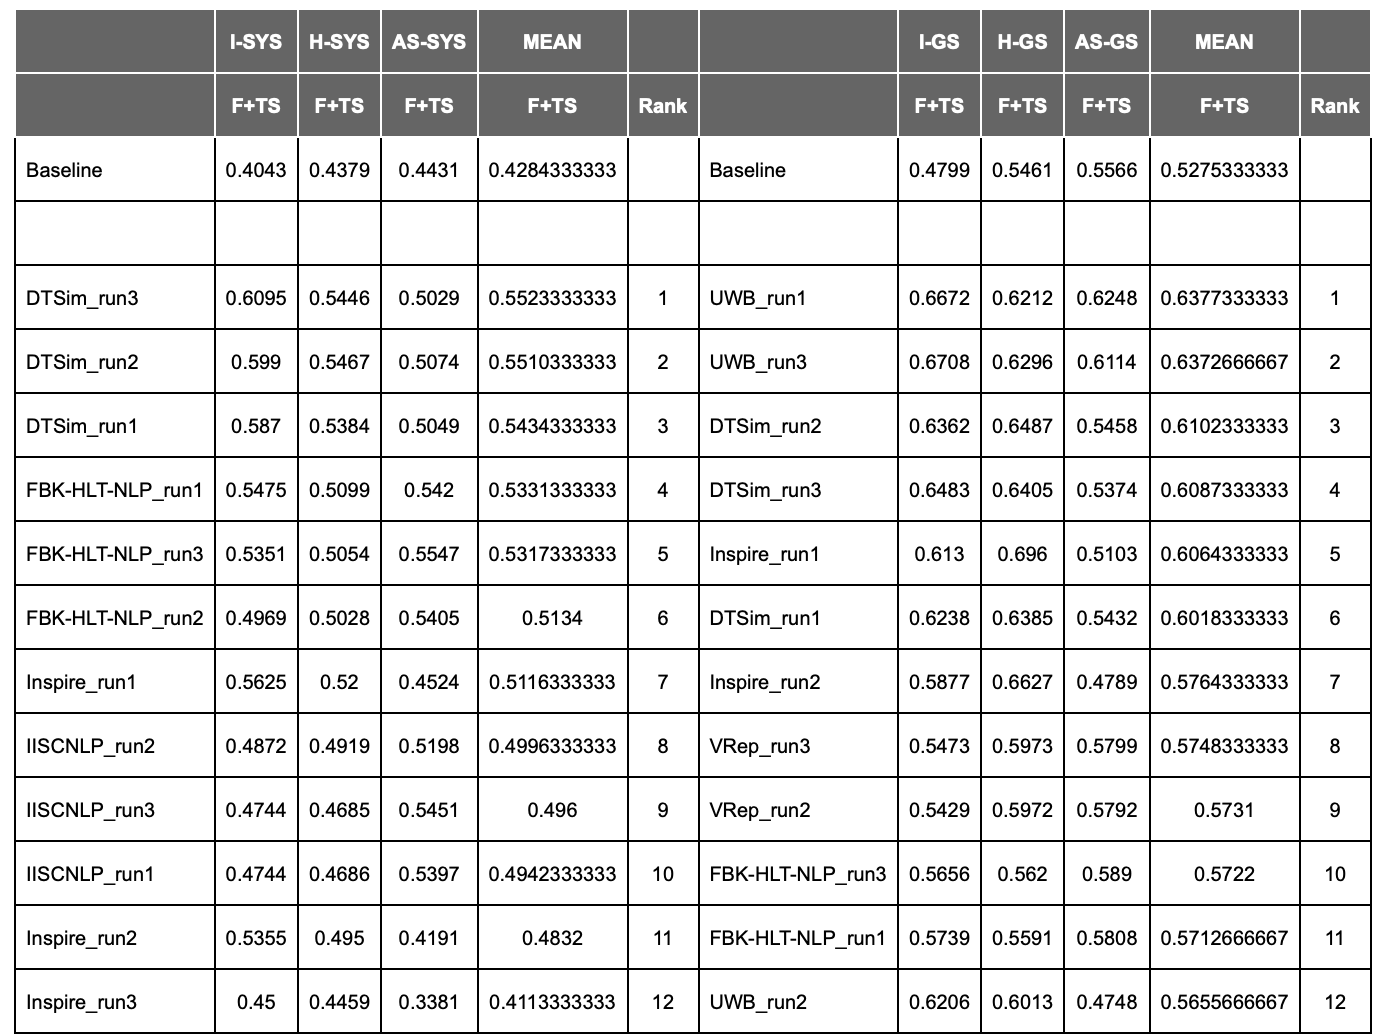
\includegraphics[width=16cm,angle=0]{truncated_results.png}
\begin{figure}[!h]
\caption{Résultats (tronqués) de la \og shared task \fg{}}
\end{figure}
 \end{center}


    \subsection{Cadre expérimental}

        \subsubsection{Description des données}

 [Insérer paragraphe sur les données]

        \subsubsection{Approche empirique}

    \paragraph{Identification des segments}
    \hfill \break
    \textit{En entrée}: deux fichiers. Le premier contient les premières phrases de chaque paire. Le second contient les deuxièmes phrases de chaque paire. \hfill \break
    \textit{En sortie}: deux fichiers. Le premier contient les premières phrases de chaque paire avec des '[' et ']' pour marquer les segments. Le second contient les deuxièmes phrases de chaque paire avec des '[' et ']' pour marquer les segments.

 \paragraph{Alignement et score de similarité}
    \hfill \break
    \textit{En entrée}: deux fichiers. Le premier contient les premières phrases de chaque paire avec des '[' et ']' pour marquer les segments. Le second contient les deuxièmes phrases de chaque paire avec des '[' et ']' pour marquer les segments. \hfill \break
    \textit{En sortie}: Un fichier .wa (de type xml) qui, pour une ligne par alignement, contient l'indice d'un token de la première phrase d'une paire, l'indice d'un token de la deuxième phrase de la paire et le score de similarité associé.



    \subsection{Baseline}

    Dans cette section, nous décrivons les différentes briques du système baseline que nous avons implémenter afin de résoudre notre tâche.

    \subsubsection{Tokenisation et plongement lexical}

Tout d’abord, on cherche à standardiser les données brutes pour les rendre plus faciles d'utilisation : c’est la phase de \og preprocessing \fg{}. On supprime les éléments qui ne sont pas nécessaires à l’analyse d’une phrase, par exemple, les ponctuations telles que \og , \fg{}, \og ; \fg{} ou bien \og - \fg{}. Tous les mots sont aussi passés en minuscule. Ensuite, vient la tokenisation. On sépare les mots d’une phrase en ce qu'on appelle des \og tokens \fg{}. Cela nous permet de travailler individuellement sur chaque mot.
Cependant, un ordinateur ne peut pas réaliser de calculs sur une chaîne de caractères. L’embedding pallie ce problème en transformant un mot en un vecteur. Nous choisissons d’utiliser des vecteurs de dimension 100. On pourrait entraîner un embedding par nous-même, mais ce n’est pas le cœur de notre sujet, c'est pourquoi on préfère utiliser des embeddings pré-entraînés. Il existe trois embeddings faciles à utiliser : \textit{Word2Vec}, \textit{GloVe} et \textit{FastText}. Pour le système de base, on choisit \textit{GloVe}, mais dans une version plus avancée, on pourra réaliser plusieurs embeddings et choisir celui donnant le meilleur résultat. On obtient finalement chaque mot de nos données sous forme vectorielle pouvant être lu et exploité facilement par notre réseau de neurones.

 \paragraph{POS-tagging}

Dans une optique d’amélioration de notre segmentation et de développement d'un modèle multimodal, nous avons pensé que l’ajout d’un \og POS-tagging \fg{} aux caractéristiques d’entrée de notre modèle pourrait être intéressant. Nous avons donc utilisé l’API \textit{NLTK} pour effectuer un étiquetage automatique à partir des phrases tokenisées de la base de données. Ces nouvelles caractéristiques ne sont pas encore utilisées dans notre modèle, mais sont prêtes si besoin.

    \subsubsection{Création de segments}
 Afin de réaliser la segmentation des phrases, nous avons créé un modèle afin de prédire et délimiter les unités de sens dans une phrase. À l’aide de ce modèle, nous cherchons à réaliser l'encodage BIO d’une phrase, c’est-à-dire prédire un label pour chaque mot de la phrase parmi ‘B’ (Begin), ‘I’ (Inside) ou ‘O’ (Outside) ; ces significations faisant référence à l’appartenance du mot à une unité de sens. Nous avons fait le choix d’un modèle récursif de type \og Simple RNN \fg{}. Les étiquettes nous permettent ensuite de délimiter les segments de la phrase avant de passer à l’étape de leur alignement.

Les données en entrée du réseau récurrent correspondent à des représentations vectorielles (issues d’une couche d’embeddings de GloVe) des mots d’une phrase, initialement tokenisés. Les étiquettes utilisées pour l'entraînement correspondent aux représentations \og one-hot  \fg{} des étiquettes BIO (encodées 0, 1, 2) de chacun des mots des phrases déjà segmentées mises à disposition dans le set de données du concours SemEval.

 \paragraph{Remarques :}
 Même si le modèle n’a pas à prédire d’étiquette ‘O’ pour un mot de la phrase, on lui laisse la possibilité de le faire uniquement afin de pouvoir ajouter une classe \og padding \fg{} qui nous permettra d’uniformiser la taille des phrases du dataset en entrée du modèle.

De plus, il faut être vigilant lors de l’évaluation de la précision du modèle, car il ne faut pas prendre en compte la performance du modèle quant à la prédiction du \og padding \fg{} à la fin de la phrase. Ainsi, afin d’évaluer le score pour une phrase, nous partons des prédictions de fin de phrase et commençons à calculer le score à partir du moment ou la vraie étiquette est différente de ‘O’ (c'est-à-dire le moment où il ne s’agit plus d'étiquettes associées au \og padding \fg{}, car il n’y a pas de labels ‘O’ présents à l’origine dans notre dataset.)

Enfin, les améliorations à apporter à notre modèle sont la prise en compte, lors de l’entraînement, qu’une diminution du \textit{loss} lié à la capacité de prédiction du \og padding \fg{} n’est pas l’important pour le modèle. Nous aimerions pouvoir déterminer quand stopper l’entraînement avant de sur-apprendre le \og padding \fg{}. Nous ne pouvons pas mettre en place de solution de régularisation classique, car le \og padding \fg{} a été créé comme une étiquette à prédire pour le modèle.

\subsubsection{Alignement des segments}

En s’inspirant des modèles de Banjade et al. \cite{banjade}  \cite{banjadeautre}, nous utilisons la méthode de Kuhn-Munkres pour optimiser l’alignement entre les mots puis l’alignement entre les segments et obtenir une similarité globale maximale. La similarité d’un segment ou d’une phrase est calculée en faisant la somme des similarités des éléments le constituant une fois ces derniers alignés de manière optimale. Pour cela, nous utilisons la fonction \og linear\_sum\_assignment \fg{} de la bibliothèque \textit{scipy.optimize}. Cette fonction prend en entrée une matrice $M$ telle que $M_{ij}$ correspond à la similarité de l’élément i du 1er segment ou phrase et de l’élément j du 2nd segment ou phrase et renvoie la combinaison de coefficients des deux segments ou phrases optimisant la similarité globale. On utilise tout d’abord cette fonction sur les segments 2 par 2. On cherche donc à aligner les mots de ces 2 segments de manière optimale pour déterminer leur similarité.

 On remplit la matrice $M$ en calculant la similarité du cosinus entre deux mots avec la formule suivante :
 \begin{equation}
    sim(mot_{1}, mot_{2})=\frac{\langle mot_{1}, mot_{2}\rangle}{|mot_{1}||mot_{2}|}
 \end{equation}
 Avec au numérateur, le produit scalaire entre les deux mots et au dénominateur, le produit de leurs normes. Une fois la combinaison des coefficients optimaux renvoyée par la fonction \og linear\_sum\_assignment \fg{}, on peut calculer la similarité entre les deux segments comme la somme des similarités mot à mot. On utilise ensuite la fonction \og linear\_sum\_assignment \fg{} sur deux phrases. On cherche cette fois-ci à aligner les segments de ces deux phrases de manière optimale et obtenir un score de similarité entre 0 et 5 pour des segments alignés. L’étape ci-dessus nous permet de remplir la matrice $M^{\prime}$ telle que $M^{\prime}_{ij}$ correspond à la similarité entre le segment i de la phrase 1 et le segment j de la phrase 2. Nous obtenons en sortie de la fonction la combinaison des coefficients optimaux ce qui nous permet de calculer un score de similarité entre deux segments alignés. Pour obtenir un score entre 0 et 5, on peut effectuer un \og minmaxscaling \fg{} sur les coefficients de similarités des segments alignés des deux phrases puis multiplier les valeurs obtenues par 5.

N.B. : si les matrices $M$ et $M^{\prime}$ ont plus de lignes que de colonnes alors certaines combinaisons ne seront pas testées pour trouver la solution optimale.
Il faut donc faire attention à ce que le premier argument de la fonction \og linear\_sum\_assignment \fg{} soit toujours l’élément de plus petite taille.

 \subsubsection{Analyse des résultats}

 En testant notre modèle sur des phrases issues de \textit{STSint.input.headlines}, on remarque que notre modèle renvoie uniquement 3 valeurs de score de similarité entre deux segments : 0, 2 et 5. Ceci est notamment dû au fait que les scores de similarité entre deux segments sont modifiés pour obtenir un score entre 0 et 5 : on fait un \textit{min-max scaling} des scores, puis on les multiplie par 5 et on les arrondit enfin à l'entier le plus proche.

 Si on regarde les paires de phrases ayant un score de similarité au moins égal à 5, on note que ces scores sont obtenus pour des segments de grande taille (au moins trois tokens). Ainsi, notre modèle va considérer que deux segments de grande taille sont très similaires peu importe leur relation. Il faudrait donc rajouter un terme de normalisation dans nos calculs de similarité en divisant, par exemple, par la taille du plus grand des deux segments.

Dans l'exemple ci-dessous, le score entre \og [ four suspected militants ] \fg{} et \og [ in Russia coal mine blast ]  \fg{} vaut 5 tandis que les autres scores sont nuls alors que [kills] et [killed] devraient avoir un score de similarité proche de 5. On remarque cependant que \og [ kills ] \fg{} et \og [ killed ] \fg{} ont bien été alignés :
\begin{eqnarray*}
\textbf{Phrase 1 : [ Drone strike ] [ kills ] [ four suspected militants ] [ in Pakistan ]}\\
\textbf{Phrase 2 : [ Ten ] [ killed ] [ in Russia coal mine blast ]}\\
\textrm{[ kills ] <-> [ killed ] (score 0)}\\
\textrm{[ four suspected militants ] <-> [ in Russia coal mine blast ] (score 5)}\\
\textrm{[in Pakistan] <-> [Ten] (score 0)}
\end{eqnarray*}


De même, on voit que le score de similarité le plus important (score 5 entre \og [ four suspected militants ] \fg{} et \og [ as Maracana re-opens ]\fg{}) correspond aux deux segments les plus grands :
\begin{eqnarray*}
\textbf{Phrase 1 : [ Drone strike ] [ kills ] [ four suspected militants ] [ in Pakistan ]}\\
\textbf{Phrase 2 : [ Brazil ] [ held ] [ by England ] [ 2-2 ] [ as Maracana re-opens ]}\\
\textrm{[ Drone strike ] <-> [ by England ] (score 2)}\\
\textrm{[ kills ] <-> [ 2-2 ] (score 0)}\\
\textrm{[ four suspected militants ] <-> [ as Maracana re-opens ] (score 5)}\\
\textrm{[in Pakistan] <-> [held] (score 0)}
\end{eqnarray*}

    \subsection{Modèle proposé}
     Ce qui est difficile, c’est de prendre en compte la variabilité dans les façons d’exprimer des informations dans des phrases similaires. Cette tâche date d’avant l’adoption généralisée de modèles neuronaux comme BERT. Dans un second temps, nous proposerons donc une solution qui met à profit notamment les embedding et tokenizer mis à disposition dans les librairies transformers.

 \subsubsection{Architecture}
 Lien vers le code-source du modèle : \href{https://github.com/timfronteau/Semantic_chunk_identification}{CLIQUER ICI !}
 \subsubsection{Ressources supplémentaires}

 \subsection{Analyse des résultats obtenus}
 \subsubsection{Évaluation}
 \paragraph{En théorie}
 \paragraph{Dans les faits}


 \subsubsection{Points forts / faibles}
 Un des points forts de notre modèle est qu'il utilise le modèle de segmentation de \textit{BERT} qui a été pré-entraîné sur des millions de données. Ceci nous permet d'avoir un modèle plus performant et plus généraliste qu'un modèle de segmentation uniquement entraîné sur nos données.

Concernant les points faibles de notre approche, le système d'alignement des segments les plus proches ne fonctionne pas pour le moment pour tous les segments et nous avons pu voir dans les résultats de notre système de base, que l'alignement de certains segments de même longueur est favorisé par notre modèle peu importe le contenu des segments.

La correction de ces dysfonctionnements serait une piste d'amélioration si l'on avait plus de temps pour continuer à améliorer le projet.
 \subsubsection{Perspectives}
 \paragraph{Segments comparables}
       \hfill \break
En nous inspirant de \cite{banjade}, nous allons introduire des règles dans l’alignement des segments pour aligner uniquement ceux qui sont \og comparables \fg{} et ainsi améliorer les performances de notre modèle à l'état de l'art. En effet, nous avons remarqué, après avoir fait un \og embedding \fg{} en utilisant \textit{SentenceTransformer}, que les tokens \og 12 \fg{} et \og amour \fg{} ont une similarité du cosinus plus élevée que les tokens \og amour \fg{} et  \og haine \fg{}. Ceci est contre-intuitif étant donné que \og amour \fg{} et \og haine \fg{} sont tous les deux des noms communs et appartiennent à la même thématique contrairement aux deux premiers. C'est peut-être dû au fait qu'ils sont antonymes l’un de l’autre, mais les similarités du cosinus sont toutes les deux positives ce qui contredit cette hypothèse.

Pour remédier à ce problème qui pourrait grandement diminuer les performances de notre modèle, nous décidons donc d’uniquement aligner les segments correspondant au même type d’entité NER. Pour cela, nous utilisons la variable \textit{entity\_group} renvoyée pour chaque segment par notre modèle.

 Une autre piste d'amélioration serait d'ajuster (fine-tuner) le modèle de segmentation de BERT sur nos données d'entraînement pour obtenir de meilleures performances.
    \printbibliography
\end{document}